\documentclass{article}

\usepackage{graphicx}
\usepackage{tikz}
\usepackage{tikzsymbols}
\usetikzlibrary{calc,patterns,shapes.geometric}
\pagestyle{empty}
\usepackage[margin=0pt]{geometry}
\geometry{papersize={14in,12in}}

\def\centerarc[#1](#2)(#3:#4:#5){\draw[#1] ($(#2)+({#5*cos(#3)},{#5*sin(#3)})$) arc (#3:#4:#5);}

\begin{document}
	\begin{figure}
		\centering
		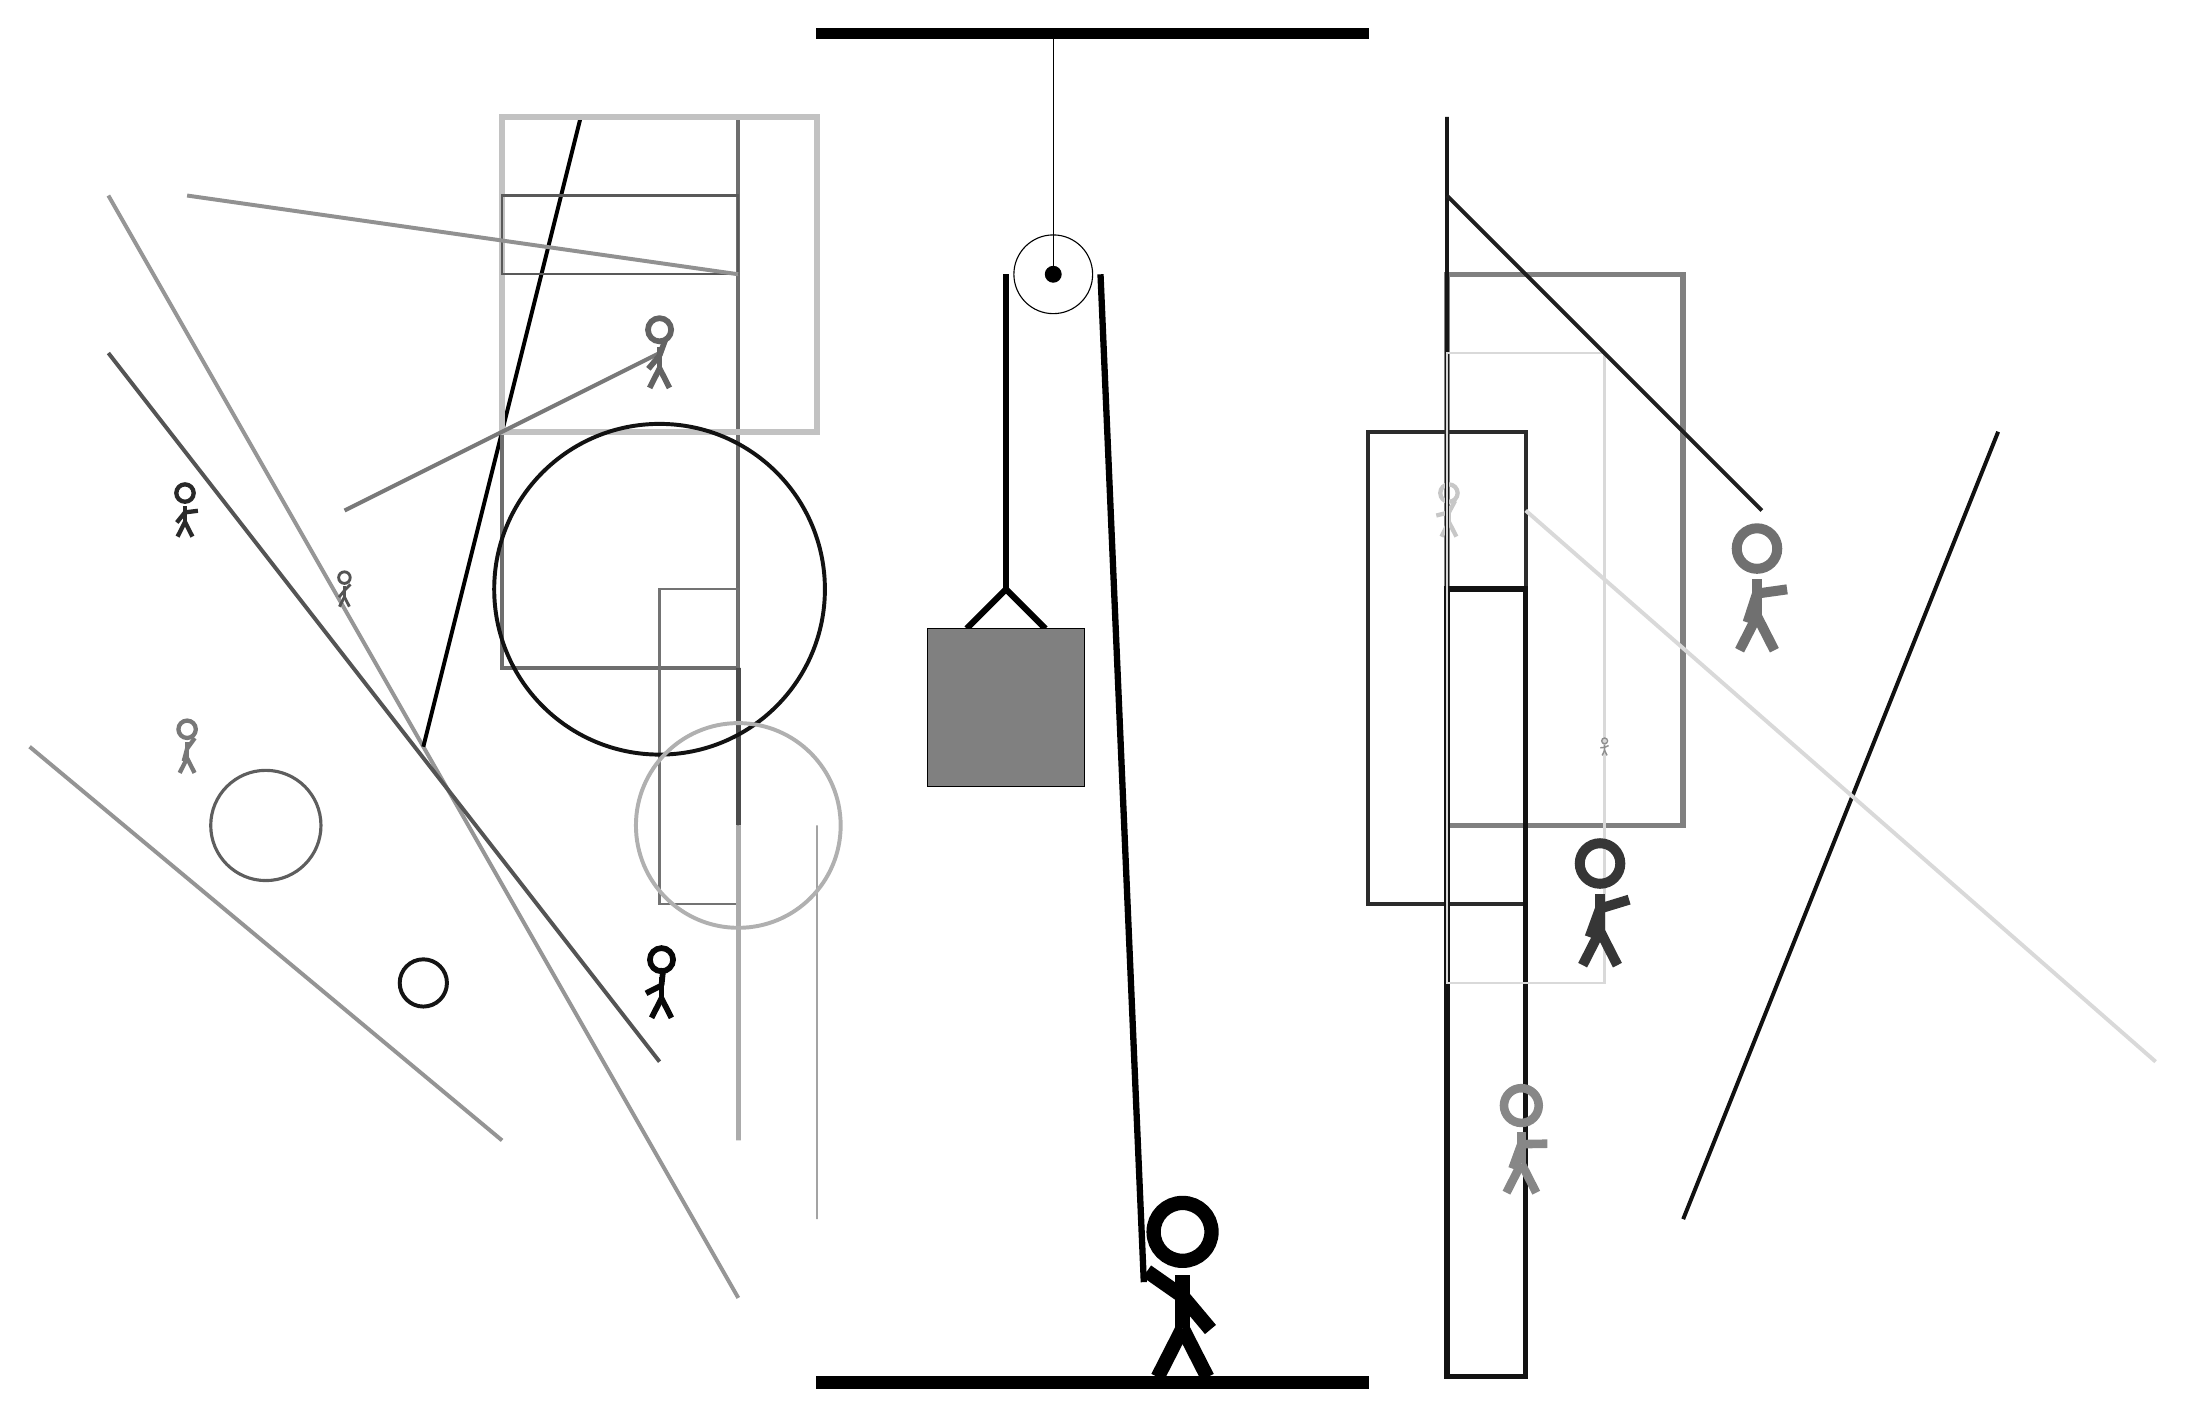
\begin{tikzpicture}
			%%%%% START %%%%%
			
			\draw[fill=black] (-2, 14) rectangle (5, 14.125);
			
			\draw[line width=0.7mm, color=black!50] (6, 4) rectangle (9, 11);
			
			\draw[line width=0.5mm, color=black!41](-3, -2) -- (-11, 12);
			\draw[line width=0.5mm, color=black!100](-5, 13) -- (-7, 5);
			\draw[line width=0.5mm, color=black!57] (-3, 6) rectangle (-6, 13);
			\node[line width=0.4mm, color=black!22] at (6, 8) {\Strichmaxerl[3][14][62]};
			
			\draw[line width=0.5mm, color=black!93](9, -1) -- (13, 9);
			
			\draw [line width=0.4mm, color=black!63](-9, 4) circle (0.7);
			\draw[line width=0.4mm, color=black!91] (6, 13) rectangle (6, 2);
			\draw[line width=0.2mm, color=black!29] (-3, 11) rectangle (-3, 12);
			
			\draw[line width=0.3mm, color=black!55] (-3, 3) rectangle (-4, 7);
			
			\draw[line width=0.7mm, color=black!24] (-2, 13) rectangle (-6, 9);
			
			\node[line width=0.2mm, color=black!84] at (-10, 8) {\Strichmaxerl[3][51][7]};
			\draw[line width=0.5mm, color=black!83] (5, 3) rectangle (7, 9);
			
			\draw[line width=0.5mm, color=black!67](-4, 1) -- (-11, 10);
			\draw[line width=0.7mm, color=black!93] (6, 7) rectangle (7, -3);
			\draw[line width=0.7mm, color=black!70] (-3, 4) rectangle (-3, 6);
			\draw[line width=0.3mm, color=black!65] (-3, 12) rectangle (-6, 11);
			\node[line width=0.7mm, color=black!53] at (-10, 5) {\Strichmaxerl[3][75][54]};
			\draw[line width=0.5mm, color=black!15](7, 8) -- (15, 1);
			\draw[line width=0.3mm, color=black!15] (6, 2) rectangle (8, 10);
			\draw[line width=0.3mm, color=black!36] (-2, -1) rectangle (-2, 4);
			\draw[line width=0.6mm, color=black!33] (-3, 4) rectangle (-3, 0);
			\draw[line width=0.5mm, color=black!88](6, 12) -- (10, 8);
			\node[line width=0.3mm, color=black!56] at (10, 7) {\Strichmaxerl[7][72][8]};
			\node[line width=0.7mm, color=black!67] at (-8, 7) {\Strichmaxerl[2][51][45]};
			
			\node[line width=0.6mm, color=black!97] at (-4, 2) {\Strichmaxerl[4][27][84]};
			
			\node[line width=0.7mm, color=black!44] at (8, 5) {\Strichmaxerl[1][6][24]};
			\draw[line width=0.5mm, color=black!42](-6, 0) -- (-12, 5);
			\draw [line width=0.5mm, color=black!93](-4, 7) circle (2.1);
			\draw [line width=0.5mm, color=black!92](-7, 2) circle (0.3);
			\draw[line width=0.5mm, color=black!53](-4, 10) -- (-8, 8);
			
			\node[line width=0.5mm, color=black!47] at (7, 0) {\Strichmaxerl[6][70][1]};
			\node[line width=0.7mm, color=black!61] at (-4, 10) {\Strichmaxerl[4][50][70]};
			\draw[line width=0.5mm, color=black!43](-3, 11) -- (-10, 12);
			\node[line width=0.4mm, color=black!79] at (8, 3) {\Strichmaxerl[7][70][17]};
			\draw [line width=0.5mm, color=black!31](-3, 4) circle (1.3);
			
			\draw (1, 11) circle (0.5);
			\draw[fill=black] (1, 11) circle (0.1);
			\draw (1, 14) -- (1, 11);
			
			\draw[line width=0.8mm] (-0.1, 6.5) -- (0.4, 7.0) -- (0.9, 6.5);
			\draw[fill=black!50] (-0.6, 6.5) rectangle (1.4, 4.5);
			
			\draw[line width=0.8mm] (0.4, 11) -- (0.4, 7.0);
			\centerarc[line width=0.8mm](1, 11)(0:180:0.6);
			\draw[line width=0.8mm](1.6, 11) -- (2.15, -1.8);
			
			\node at (2.6, -1.9) {\Strichmaxerl[10][-35][-50]};
			
			\draw[fill=black] (-2, -3) rectangle (5, -3.15);
			
			%%%%% END %%%%%
		\end{tikzpicture}
	\end{figure}	
\end{document}